% Source PDF page 355 (printed p. 341)
如果 (6.25) 可行，至少存在一个这样的效用函数；事实上，由可行的 $u_1,\ldots,u_m,g_1,\ldots,g_m$ 还能构造一个分段线性效用函数。如果 (6.25) 不可行，就能断定：不存在与给定严格和非严格偏好集合一致的凹递增效用函数。

例如，假设已知消费者偏好 $\mathcal P$、$\mathcal P_{\rm weak}$ 与至少一个凹递增效用函数一致。考虑不属于 $\mathcal P$ 或 $\mathcal P_{\rm weak}$ 的一对 $(k,l)$，即篮子 $k$ 与 $l$ 之间的消费者偏好尚不明确。在某些情况下，即使不知道背后的偏好函数，也能推出二者之间的偏好。为此，在已知偏好 (6.22) 中加入不等式 $u(a_k)\le u(a_l)$，表示篮子 $l$ 比 $k$ 更受偏好，或两者同样有吸引力。然后求解包含额外弱偏好 $u(a_k)\le u(a_l)$ 的线性规划可行性问题 (6.25)。如果扩充后的偏好集合不可行，就意味着：任何与原始给定消费者偏好数据一致的凹不减效用函数，都必须满足 $u(a_k)>u(a_l)$。换言之，无须知道背后的效用函数，就能断定消费者更喜欢篮子 $k$ 而不是 $l$。

\begin{origexample}{6.9}
下面用一个简单数值例子说明上述讨论。考虑由两种商品组成的篮子，以便画出这些篮子。为生成消费者偏好数据 $\mathcal P$，在 $[0,1]^2$ 中随机生成40个点，然后用效用函数
\[u(x_1,x_2)=(1.1x_1^{1/2}+0.8x_2^{1/2})/1.9\]
比较它们。图6.25给出这些商品篮子以及效用函数 $u$ 的几条等值线。

现在，只用消费者偏好数据，当然不使用真实效用函数 $u$，将这40个篮子逐一与篮子 $a_0=(0.5,0.5)$ 比较。对每个原始篮子 $a_i$，求解上面描述的线性规划可行性问题，检查能否断定消费者更喜欢 $a_0$ 而非 $a_i$。同样，检查能否断定 $a_i$ 比 $a_0$ 更受偏好。对每个 $a_i$，有三种可能结果：确定更喜欢 $a_0$，确定更喜欢 $a_i$，或两个 LP 可行性问题均可行、因而无法作出结论。（这里“确定更喜欢”表示：对于任何与原始给定数据一致的凹不减效用函数，该偏好都成立。）

结果表明，与 $(0.5,0.5)$ 相比，21个篮子确定被排除，14个篮子确定更受偏好；依据消费者偏好数据，对剩余5个篮子无法作出结论。结果见图6.26。注意，仅用效用函数的单调性就能断定：$(0.5,0.5)$ 下方和左方的篮子会被排除，选择 $(0.5,0.5)$；同样，位于其上方和右方的点必定更受偏好。因此，对这17个点，无须求解可行性 LP (6.25)。不过，对另外两个象限中的23个点分类，需要使用凹性假设并求解可行性 LP (6.25)。
\end{origexample}

% Source PDF page 356 (printed p. 342)
\begin{figure}[htbp]\centering
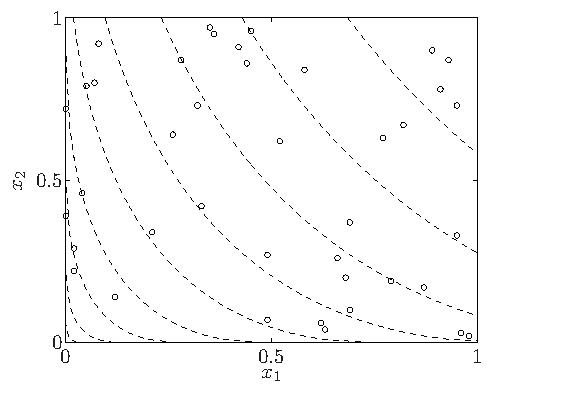
\includegraphics[width=.68\textwidth]{ch06-25.pdf}
\caption*{图6.25\quad 40个商品篮子 $a_1,\ldots,a_{40}$，以圆圈表示。虚线是真实效用函数 $u$ 的 $0.1,0.2,\ldots,0.9$ 等值线。利用该效用函数确定40个篮子之间的消费者偏好数据 $\mathcal P$。}
\end{figure}
\begin{figure}[htbp]\centering
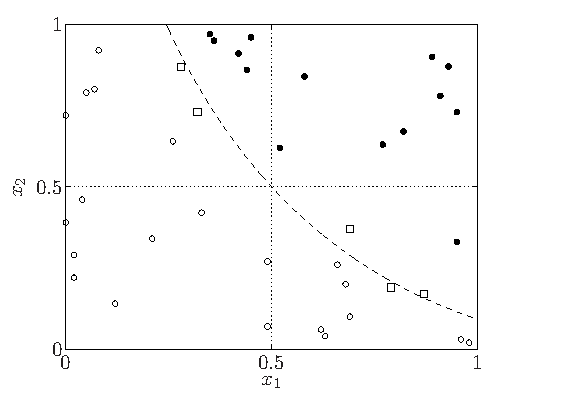
\includegraphics[width=.68\textwidth]{ch06-26.pdf}
\caption*{图6.26\quad 对新商品篮子 $a_0=(0.5,0.5)$，采用 LP (6.25) 进行消费者偏好分析的结果。若原始篮子确定被排除（$u(a_k)<u(a_0)$），画为空心圆；若确定更受偏好（$u(a_k)>u(a_0)$），画为实心黑圆；若无法作出结论，画为方框。经过 $(0.5,0.5)$ 的真实效用函数等值线用虚线表示。穿过 $(0.5,0.5)$ 的水平线和竖直线将 $[0,1]^2$ 划为四个象限。根据 $u$ 的单调性，右上象限中的点一定比 $(0.5,0.5)$ 更受偏好；同样，$(0.5,0.5)$ 一定比左下象限中的点更受偏好。对另外两个象限中的点，结果并不明显。}
\end{figure}

% Source PDF page 357 (printed p. 343)
\section*{文献说明}
\addcontentsline{toc}{section}{文献说明}
Huber [Hub64, Hub81] 分析了不同惩罚函数逼近的稳健性，并提出惩罚函数 (6.4)。对数障碍惩罚函数出现在控制理论中，用于系统闭环频率响应，有多种名称，例如 central $H_\infty$ 或 risk-averse control；见 Boyd 与 Barratt [BB91] 及其中的参考文献。

许多书籍讨论正则化逼近，包括 Tikhonov 与 Arsenin [TA77]、Hansen [Han98]。Tikhonov 正则化有时称为\emph{岭回归}（Golub 与 Van Loan [GL89, 第564页]）。采用 $\ell_1$ 范数正则化的最小二乘逼近，也称为 \emph{lasso}（Tibshirani [Tib96]）。Hastie、Tibshirani 与 Friedman [HTF01, 第3.4节] 讨论并比较了其他最小二乘正则化和回归向量选择方法。

Rudin、Osher 与 Fatemi [ROF92] 为图像重构引入了全变差去噪。

El Ghaoui 与 Lebret [EL97]，以及 Chandrasekaran、Golub、Gu 与 Sayed [CGGS98]，提出了范数有界不确定性下的稳健最小二乘问题（第321页）。El Ghaoui 与 Lebret 还给出了具有结构化不确定性的稳健最小二乘问题的 SDP 表述（第323页）。

Chen、Donoho 与 Saunders [CDS01] 讨论通过线性规划进行基追踪，并将 $\ell_1$ 范数正则化问题 (6.18) 称为\emph{基追踪去噪}。Meyer 与 Pratt [MP68] 是研究效用函数求界问题的一篇早期论文。

% Source PDF page 358 (printed p. 344)
\section*{习题}
\addcontentsline{toc}{section}{习题}
\subsection*{范数逼近与最小范数问题}
\paragraph{6.1} \emph{对数障碍惩罚的二次界。}令 $\phi:\R\to\R$ 为限制值 $a>0$ 的对数障碍惩罚函数：
\[\phi(u)=\begin{cases}-a^2\log(1-(u/a)^2),&|u|<a,\\\infty,&\text{其他情形}.\end{cases}\]
证明：若 $u\in\R^m$ 满足 $\norm u_\infty<a$，则
\[\norm u_2^2\le\sum_{i=1}^m\phi(u_i)\le\frac{\phi(\norm u_\infty)}{\norm u_\infty^2}\norm u_2^2.\]
这意味着，如果 $\norm u_\infty$ 相对于 $a$ 较小，$\norm u_2^2$ 就很好地近似 $\sum_{i=1}^m\phi(u_i)$。例如，若 $\norm u_\infty/a=0.25$，则
\[\norm u_2^2\le\sum_{i=1}^m\phi(u_i)\le1.033\cdot\norm u_2^2.\]

\paragraph{6.2} \emph{用常向量作 $\ell_1$、$\ell_2$ 和 $\ell_\infty$ 范数逼近。}对于只有一个标量变量 $x\in\R$ 的范数逼近问题
\[\text{最小化}\quad\norm{x\one-b},\]
采用 $\ell_1$、$\ell_2$ 和 $\ell_\infty$ 范数时，其解分别是什么？

\paragraph{6.3} 将下列逼近问题表述为 LP、QP、SOCP 或 SDP。问题数据为 $A\in\R^{m\times n}$ 和 $b\in\R^m$，$A$ 的各行记为 $a_i^\T$。
\begin{enumerate}[label=(\alph*)]
\item \emph{死区线性惩罚逼近：}最小化 $\sum_{i=1}^m\phi(a_i^\T x-b_i)$，其中
\[\phi(u)=\begin{cases}0,&|u|\le a,\\|u|-a,&|u|>a,\end{cases}\]
且 $a>0$。
\item \emph{对数障碍惩罚逼近：}最小化 $\sum_{i=1}^m\phi(a_i^\T x-b_i)$，其中
\[\phi(u)=\begin{cases}-a^2\log(1-(u/a)^2),&|u|<a,\\\infty,&|u|\ge a,\end{cases}\]
且 $a>0$。
\item \emph{Huber 惩罚逼近：}最小化 $\sum_{i=1}^m\phi(a_i^\T x-b_i)$，其中
\[\phi(u)=\begin{cases}u^2,&|u|\le M,\\M(2|u|-M),&|u|>M,\end{cases}\]
且 $M>0$。
\item \emph{对数 Chebyshev 逼近：}最小化 $\max_{i=1,\ldots,m}|\log(a_i^\T x)-\log b_i|$，假定 $b\succ0$。一个等价的凸形式为
\[\begin{array}{ll}\text{最小化}&t\\\text{约束条件}&1/t\le a_i^\T x/b_i\le t,\quad i=1,\ldots,m,\end{array}\]
变量为 $x\in\R^n$、$t\in\R$，定义域为 $\R^n\times\R_{++}$。
\end{enumerate}

% Source PDF page 359 (printed p. 345)
\begin{enumerate}[label=(\alph*),start=5]
\item \emph{最小化最大的 $k$ 个残差之和：}
\[\begin{array}{ll}\text{最小化}&\displaystyle\sum_{i=1}^k|r|_{[i]}\\\text{约束条件}&r=Ax-b,\end{array}\]
其中 $|r|_{[1]}\ge|r|_{[2]}\ge\cdots\ge|r|_{[m]}$ 是将 $|r_1|,|r_2|,\ldots,|r_m|$ 按降序排列的结果。（$k=1$ 时化为 $\ell_\infty$ 范数逼近；$k=m$ 时化为 $\ell_1$ 范数逼近。）\emph{提示：}见习题5.19。
\end{enumerate}

\paragraph{6.4} \emph{$\ell_1$ 范数逼近的可微近似。}函数 $\phi(u)=(u^2+\epsilon)^{1/2}$，其中参数 $\epsilon>0$，有时用作绝对值函数 $|u|$ 的可微近似。为了近似求解 $\ell_1$ 范数逼近问题
\begin{equation}\text{最小化}\quad\norm{Ax-b}_1,\tag{6.26}\end{equation}
其中 $A\in\R^{m\times n}$，转而求解问题
\begin{equation}\text{最小化}\quad\sum_{i=1}^m\phi(a_i^\T x-b_i),\tag{6.27}\end{equation}
其中 $a_i^\T$ 是 $A$ 的第 $i$ 行。假设 $\rank A=n$。

令 $p^\star$ 为 $\ell_1$ 范数逼近问题 (6.26) 的最优值，$\widehat x$ 为近似问题 (6.27) 的最优解，$\widehat r$ 为对应残差，$\widehat r=A\widehat x-b$。
\begin{enumerate}[label=(\alph*)]
\item 证明 $p^\star\ge\sum_{i=1}^m\widehat r_i^2/(\widehat r_i^2+\epsilon)^{1/2}$。
\item 证明
\[\norm{A\widehat x-b}_1\le p^\star+\sum_{i=1}^m|\widehat r_i|\left(1-\frac{|\widehat r_i|}{(\widehat r_i^2+\epsilon)^{1/2}}\right).\]
\end{enumerate}
（计算 $\widehat x$ 后求出右端，就得到 $\widehat x$ 对 $\ell_1$ 范数逼近问题的次优程度的一个界。）

\paragraph{6.5} \emph{最短长度逼近。}考虑问题
\[\begin{array}{ll}\text{最小化}&\operatorname{length}(x)\\\text{约束条件}&\norm{Ax-b}\le\epsilon,\end{array}\]
其中 $\operatorname{length}(x)=\min\{k\mid x_i=0\text{ 对 }i>k\}$。问题变量为 $x\in\R^n$，参数为 $A\in\R^{m\times n}$、$b\in\R^m$、$\epsilon>0$。在回归中，要求按原有顺序取尽可能少的 $A$ 的列，以在误差 $\epsilon$ 内逼近向量 $b$。

证明这是一个拟凸优化问题。

\paragraph{6.6} \emph{一些惩罚函数逼近问题的对偶。}对于以下惩罚函数 $\phi:\R\to\R$，推导问题
\[\begin{array}{ll}\text{最小化}&\displaystyle\sum_{i=1}^m\phi(r_i)\\\text{约束条件}&r=Ax-b\end{array}\]
的拉格朗日对偶。变量为 $x\in\R^n$、$r\in\R^m$。
\begin{enumerate}[label=(\alph*)]
\item 死区线性惩罚（死区宽度 $a=1$）：
\[\phi(u)=\begin{cases}0,&|u|\le1,\\|u|-1,&|u|>1.\end{cases}\]
\item Huber 惩罚（$M=1$）：
\[\phi(u)=\begin{cases}u^2,&|u|\le1,\\2|u|-1,&|u|>1.\end{cases}\]
\end{enumerate}

% Source PDF page 360 (printed p. 346)
\begin{enumerate}[label=(\alph*),start=3]
\item 对数障碍（限制值 $a=1$）：
\[\phi(u)=-\log(1-u^2),\qquad\dom\phi=(-1,1).\]
\item 相对 $1$ 的偏差：
\[\phi(u)=\max\{u,1/u\}=\begin{cases}u,&u\ge1,\\1/u,&u\le1,\end{cases}\]
其中 $\dom\phi=\R_{++}$。
\end{enumerate}

\subsection*{正则化与稳健逼近}
\paragraph{6.7} \emph{采用欧几里得范数的双准则优化。}考虑双准则优化问题
\[\text{相对于 }\R_+^2\text{ 最小化}\quad(\norm{Ax-b}_2^2,\norm x_2^2),\]
其中 $A\in\R^{m\times n}$ 的秩为 $r$，$b\in\R^m$。说明如何从 $A$ 的奇异值分解
\[A=U\diag(\sigma)V^\T=\sum_{i=1}^r\sigma_i u_i v_i^\T\]
求出以下各问题的解（见第A.5.4节）。
\begin{enumerate}[label=(\alph*)]
\item Tikhonov 正则化：最小化 $\norm{Ax-b}_2^2+\delta\norm x_2^2$。
\item 在 $\norm x_2^2=\gamma$ 下最小化 $\norm{Ax-b}_2^2$。
\item 在 $\norm x_2^2=\gamma$ 下最大化 $\norm{Ax-b}_2^2$。
\end{enumerate}
其中 $\delta$ 和 $\gamma$ 是正参数。

你的结果给出计算最优权衡曲线及该双准则问题可达值集合的高效方法。

\paragraph{6.8} 将下列稳健逼近问题表述为 LP、QP、SOCP 或 SDP。对每个小题，分别考虑 $\ell_1$、$\ell_2$ 和 $\ell_\infty$ 范数。
\begin{enumerate}[label=(\alph*)]
\item 有限参数取值集合上的随机稳健逼近，即范数和问题
\[\text{最小化}\quad\sum_{i=1}^k p_i\norm{A_ix-b},\]
其中 $p\succeq0$、$\one^\T p=1$。（见第6.4.1节。）
\item 系数有界时的最坏情形稳健逼近：
\[\text{最小化}\quad\sup_{A\in\mathcal A}\norm{Ax-b},\]
其中
\[\mathcal A=\{A\in\R^{m\times n}\mid l_{ij}\le a_{ij}\le u_{ij},\ i=1,\ldots,m,\ j=1,\ldots,n\}.\]
不确定集由 $A$ 各元素的上下界描述。假设 $l_{ij}<u_{ij}$。
\item 多面体不确定性下的最坏情形稳健逼近：
\[\text{最小化}\quad\sup_{A\in\mathcal A}\norm{Ax-b},\]
其中
\[\mathcal A=\{[a_1\ \cdots\ a_m]^\T\mid C_ia_i\preceq d_i,\ i=1,\ldots,m\}.\]
给出每一行可能取值的多面体 $\mathcal P_i=\{a_i\mid C_ia_i\preceq d_i\}$ 来描述不确定性。参数 $C_i\in\R^{p_i\times n}$、$d_i\in\R^{p_i}$，$i=1,\ldots,m$ 已知。假设多面体 $\mathcal P_i$ 非空且有界。
\end{enumerate}

% Source PDF page 361 (printed p. 347)
\subsection*{函数拟合与插值}
\paragraph{6.9} \emph{极小极大有理函数拟合。}证明以下问题为拟凸问题：
\[\text{最小化}\quad\max_{i=1,\ldots,k}\left|\frac{p(t_i)}{q(t_i)}-y_i\right|,\]
其中
\[p(t)=a_0+a_1t+a_2t^2+\cdots+a_mt^m,\qquad q(t)=1+b_1t+\cdots+b_nt^n,\]
目标函数的定义域为
\[\mathcal D=\{(a,b)\in\R^{m+1}\times\R^n\mid q(t)>0,\ \alpha\le t\le\beta\}.\]
该问题用有理函数 $p(t)/q(t)$ 拟合给定数据，并要求分母多项式在区间 $[\alpha,\beta]$ 上为正。优化变量为分子、分母系数 $a_i$、$b_i$。插值点 $t_i\in[\alpha,\beta]$ 和期望函数值 $y_i$（$i=1,\ldots,k$）已知。

\paragraph{6.10} \emph{用凹、非负、不减的二次函数拟合数据。}给定数据
\[x_1,\ldots,x_N\in\R^n,\qquad y_1,\ldots,y_N\in\R,\]
希望用如下形式的二次函数拟合：
\[f(x)=(1/2)x^\T Px+q^\T x+r,\]
其中 $P\in\mathbf S^n$、$q\in\R^n$、$r\in\R$ 是模型参数，因而也是拟合问题的变量。

模型只在盒 $\mathcal B=\{x\in\R^n\mid l\preceq x\preceq u\}$ 上使用。可以假设 $l\prec u$，并且给定数据点 $x_i$ 均在该盒中。

以简单的误差平方和
\[\sum_{i=1}^N(f(x_i)-y_i)^2\]
作为拟合准则，同时对函数 $f$ 施加几个约束。首先，$f$ 必须凹。其次，$f$ 在 $\mathcal B$ 上非负，即对所有 $z\in\mathcal B$，有 $f(z)\ge0$。第三，$f$ 在 $\mathcal B$ 上不减，即当 $z,\widetilde z\in\mathcal B$ 满足 $z\preceq\widetilde z$ 时，有 $f(z)\le f(\widetilde z)$。

说明如何将该拟合问题表述为凸问题，并尽可能简化表述。

\paragraph{6.11} \emph{最小二乘方向插值。}假设 $F_1,\ldots,F_n:\R^k\to\R^p$，构造线性组合 $F:\R^k\to\R^p$：
\[F(u)=x_1F_1(u)+\cdots+x_nF_n(u),\]
其中 $x$ 是插值问题的变量。

要求 $\angle(F(v_j),q_j)=0$，$j=1,\ldots,m$，其中 $q_j$ 是给定的 $\R^p$ 中的向量，假定 $\norm{q_j}_2=1$。也就是说，要求 $F$ 在点 $v_j$ 处具有指定方向。为了确保 $F(v_j)$ 非零（为零时夹角无定义），加入最小长度约束 $\norm{F(v_j)}_2\ge\epsilon$，$j=1,\ldots,m$，其中 $\epsilon>0$ 已知。

说明如何用凸优化寻找满足上述方向及最小长度条件、并使 $\norm x_2$ 最小的 $x$。

\paragraph{6.12} \emph{用单调函数插值。}如果 $u\succeq v$ 时有 $f(u)\ge f(v)$，函数 $f:\R^k\to\R$ 就是相对于 $\R_+^k$ 单调不减的。

% Source PDF page 362 (printed p. 348)
\begin{enumerate}[label=(\alph*)]
\item 证明：存在满足 $f(u_i)=y_i$（$i=1,\ldots,m$）的单调不减函数 $f:\R^k\to\R$，当且仅当
\[u_i\succeq u_j\text{ 时有 }y_i\ge y_j,\qquad i,j=1,\ldots,m.\]
\item 证明：存在满足 $\dom f=\R^k$ 和 $f(u_i)=y_i$（$i=1,\ldots,m$）的凸单调不减函数 $f:\R^k\to\R$，当且仅当存在 $g_i\in\R^k$（$i=1,\ldots,m$），使
\[g_i\succeq0,\quad i=1,\ldots,m,\qquad y_j\ge y_i+g_i^\T(u_j-u_i),\quad i,j=1,\ldots,m.\]
\end{enumerate}

\paragraph{6.13} \emph{用拟凸函数插值。}证明：存在满足 $f(u_i)=y_i$（$i=1,\ldots,m$）的拟凸函数 $f:\R^k\to\R$，当且仅当存在 $g_i\in\R^k$（$i=1,\ldots,m$），使
\[y_j<y_i\text{ 时有 }g_i^\T(u_j-u_i)\le-1,\qquad i,j=1,\ldots,m.\]

\paragraph{6.14} [Nes00] \emph{用正实函数插值。}假设 $z_1,\ldots,z_n\in\C$ 是 $n$ 个互异点，且 $|z_i|>1$。定义 $K_{\rm np}$ 为满足下列条件的向量 $y\in\C^n$ 的集合：存在函数 $f:\C\to\C$，满足
\begin{itemize}
\item $f$ 为正实函数，即在单位圆外（$|z|>1$）解析，且实部在单位圆外非负（$|z|>1$ 时 $\operatorname{Re}f(z)\ge0$）。
\item $f$ 满足插值条件
\[f(z_1)=y_1,\qquad f(z_2)=y_2,\quad\ldots,\quad f(z_n)=y_n.\]
\end{itemize}
若正实函数集记为 $\mathcal F$，则
\[K_{\rm np}=\{y\in\C^n\mid\exists f\in\mathcal F,\ y_k=f(z_k),\ k=1,\ldots,n\}.\]
\begin{enumerate}[label=(\alph*)]
\item 可以证明，$f$ 为正实函数，当且仅当存在不减函数 $\rho$，使对所有 $|z|>1$ 有
\[f(z)=\mathrm i\operatorname{Im}f(\infty)+\int_0^{2\pi}\frac{e^{\mathrm i\theta}+z^{-1}}{e^{\mathrm i\theta}-z^{-1}}\,d\rho(\theta),\]
其中 $\mathrm i=\sqrt{-1}$（见 [KN77, 第389页]）。用这一表示证明 $K_{\rm np}$ 是闭凸锥。
\item 在向量 $x,y\in\C^n$ 之间使用内积 $\operatorname{Re}(x^{\HH}y)$，其中 $x^{\HH}$ 表示 $x$ 的共轭转置。证明 $K_{\rm np}$ 的对偶锥为
\[K_{\rm np}^*=\left\{x\in\C^n\;\middle|\;\begin{gathered}
\operatorname{Im}(\one^\T x)=0,\\
\operatorname{Re}\left(\sum_{l=1}^n x_l\frac{e^{-\mathrm i\theta}+\overline z_l^{-1}}{e^{-\mathrm i\theta}-\overline z_l^{-1}}\right)\ge0\quad\forall\theta\in[0,2\pi]
\end{gathered}\right\}.\]
\item 证明
\[K_{\rm np}^*=\left\{x\in\C^n\;\middle|\;\exists Q\in\mathbf H_+^n,\quad x_l=\sum_{k=1}^n\frac{Q_{kl}}{1-z_k^{-1}\overline z_l^{-1}},\quad l=1,\ldots,n\right\},\]
其中 $\mathbf H_+^n$ 表示所有 $n\times n$ 厄米半正定矩阵的集合。

使用以下结论，称为 Riesz--Fej\'er 定理，见 [KN77, 第60页]：形如
\[\sum_{k=0}^n(y_ke^{-\mathrm ik\theta}+\overline y_ke^{\mathrm ik\theta})\]
的函数对所有 $\theta$ 非负，当且仅当存在 $a_0,\ldots,a_n\in\C$，使
\[\sum_{k=0}^n(y_ke^{-\mathrm ik\theta}+\overline y_ke^{\mathrm ik\theta})=\left|\sum_{k=0}^n a_ke^{\mathrm ik\theta}\right|^2.\]
\end{enumerate}

% Source PDF page 363 (printed p. 349)
\begin{enumerate}[label=(\alph*),start=4]
\item 证明 $K_{\rm np}=\{y\in\C^n\mid P(y)\succeq0\}$，其中 $P(y)\in\mathbf H^n$ 定义为
\[P(y)_{kl}=\frac{y_k+\overline y_l}{1-z_k^{-1}\overline z_l^{-1}},\qquad l,k=1,\ldots,n.\]
矩阵 $P(y)$ 称为与点 $z_k,y_k$ 对应的 Nevanlinna--Pick 矩阵。

\emph{提示：}由 (a) 知，$K_{\rm np}$ 是闭凸锥，因此 $K_{\rm np}=K_{\rm np}^{**}$。
\item 作为应用，将下列问题表述为凸优化问题：
\[\begin{array}{ll}\text{最小化}&\displaystyle\sum_{k=1}^n|f(z_k)-w_k|^2\\\text{约束条件}&f\in\mathcal F.\end{array}\]
问题数据为 $n$ 个满足 $|z_k|>1$ 的点 $z_k$，以及 $n$ 个复数 $w_1,\ldots,w_n$。在所有正实函数 $f$ 上优化。
\end{enumerate}

% Source PDF page 364 (printed p. 350)
% This source page is blank.
